\section{CatBoost with Graph Features}
\label{sec:catboost_model}

This study employs the CatBoost model, a high-performance gradient boosting library, chosen specifically for its ability to handle categorical features and class imbalance effectively, as well as for its robust handling of noisy data \cite{prokhorenkova2018catboost}. CatBoost has been widely recognized for its superior performance in structured data problems, particularly when compared to other boosting algorithms like XGBoost and LightGBM, thanks to its unique techniques such as ordered boosting and categorical feature encoding. These innovations help prevent overfitting and enhance generalization in class unbalanced problems.

Here, we describe how CatBoost is combined the graph-based features that are extracted of our modeled airports network. These features are derived from the weighted directed graph and enconded as tabular features that are used as input to the model as we describe in the following sections.


\subsection{Graph Representation of the Flight Network}

\begin{figure}[ht]
    \centering
    \begin{tikzpicture}[
        ->, % directed edges
        >=stealth, % arrow tip
        node distance=3cm, % distance between nodes
        airport/.style={circle, draw, minimum size=2cm, font=\Large}, % style for airports
        flight/.style={font=\small} % style for flights
    ]

    % Nodes (Airports)
    \node[airport] (A) {SP \\ \faPlaneDeparture}; % São Paulo with departure icon
    \node[airport] (B) [right of=A] {RJ \\ \faPlaneDeparture}; % Rio de Janeiro with departure icon
    \node[airport] (C) [below of=A] {MG \\ \faPlaneDeparture}; % Minas Gerais with departure icon

    % Edges (Flights)
    \draw[->] (A) to node[flight, above] {\tikz[baseline]{\node[rotate=0]{\faPlane};}} (B); % Flight from SP to RJ, plane icon aligned (0 degrees)
    \draw[->] (B) to node[flight, right] {\tikz[baseline]{\node[rotate=220]{\faPlane};}} (C); % Flight from RJ to MG, plane icon rotated 270 degrees
    \draw[->] (C) to node[flight, left] {\tikz[baseline]{\node[rotate=96]{\faPlane};}} (A); % Flight from MG to SP, plane icon rotated 135 degrees

    \end{tikzpicture}
    \caption{Airports and Directed Flights}
    \label{fig:flight_network_graph}
\end{figure}


To model the interactions in flight data, we represented the problem as a directed graph, depicted in Figure~\ref{fig:flight_network_graph}, where each node represents an airport, here we represent the airports as states of Brazil: SP (São Paulo), MG (Minas Gerais), RJ (Rio de Janeiro). In this network:
\begin{itemize}
    \item Nodes represent airports.
    \item Directed edges represent flights, with each edge directed from the departure airport to the destination airport.
\end{itemize}
Given the frequent occurrence of multiple flights between the same pairs of airports (i.e., multiedges), we have in fact a multigraph, however we abstract it into a weighted directed graph as shown in \ref{fig:multigraph_to_weighted_graph}. Here, each edge's weight corresponds to the total number of flights between a specific pair of airports, transforming multiple directed edges into a single weighted edge. This abstraction allows us to calculate key network metrics more easily, which we then used as features in the CatBoost model.

\begin{figure}[h]
    \centering
    \begin{tikzpicture}[
        ->, % directed edges
        >=stealth, % arrow tip style
        node distance=4cm, % distance between nodes
        airport/.style={circle, draw, minimum size=2cm, font=\Large}, % style for airports
        flight/.style={font=\small, scale=0.8} % smaller size for flights
    ]
    
    % Multigraph (Left Side)
    \node[airport] (A1) {SP \\ \faPlaneDeparture}; % São Paulo with departure icon
    \node[airport] (B1) [right of=A1] {RJ \\ \faPlaneDeparture}; % Rio de Janeiro with departure icon
    \node[airport] (C1) [below of=A1, yshift=-1cm] {MG \\ \faPlaneDeparture}; % Minas Gerais with departure icon
    
    % Multiple flights in the multigraph (non-intersecting paths)
    \draw[->] (A1) to[bend left=20] node[flight, near start] {\tikz[baseline]{\node[rotate=0, scale=0.7]{\faPlane};}} (B1); % Flight 1 from SP to RJ
    \draw[->] (A1) to[bend left=40] node[flight, near start] {\tikz[baseline]{\node[rotate=0, scale=0.7]{\faPlane};}} (B1); % Flight 2 from SP to RJ
    \draw[->] (A1) to[bend left=60] node[flight, near start] {\tikz[baseline]{\node[rotate=0, scale=0.7]{\faPlane};}} (B1); % Flight 3 from SP to RJ
    
    \draw[->] (B1) to[bend right=20] node[flight, near start] {\tikz[baseline]{\node[rotate=270, scale=0.7]{\faPlane};}} (C1); % Flight 1 from RJ to MG
    \draw[->] (B1) to[bend right=40] node[flight, near start] {\tikz[baseline]{\node[rotate=270, scale=0.7]{\faPlane};}} (C1); % Flight 2 from RJ to MG
    
    \draw[->] (C1) to[bend right=20] node[flight, near start] {\tikz[baseline]{\node[rotate=135, scale=0.7]{\faPlane};}} (A1); % Flight 1 from MG to SP
    \draw[->] (C1) to[bend right=40] node[flight, near start] {\tikz[baseline]{\node[rotate=135, scale=0.7]{\faPlane};}} (A1); % Flight 2 from MG to SP
    \draw[->] (C1) to[bend right=60] node[flight, near start] {\tikz[baseline]{\node[rotate=135, scale=0.7]{\faPlane};}} (A1); % Flight 3 from MG to SP
    
    % Transformation arrow
    \node at ($(A1)!0.5!(B1)+(3.5,-2)$) {\Huge $\Rightarrow$};
    
    % Weighted Graph (Right Side)
    \node[airport] (A2) [right=6cm of A1] {SP \\ \faPlaneDeparture}; % São Paulo airport (weighted graph)
    \node[airport] (B2) [right of=A2] {RJ \\ \faPlaneDeparture}; % Rio de Janeiro airport (weighted graph)
    \node[airport] (C2) [below of=A2, yshift=-1cm] {MG \\ \faPlaneDeparture}; % Minas Gerais airport (weighted graph)
    
    % Weighted edges (single paths)
    \draw[->] (A2) to[bend left=20] node[flight, near end, yshift=0.3cm] { $W = 3$ \;} (B2); % Weighted edge from SP to RJ
    \draw[->] (B2) to[bend right=20] node[flight, near end, xshift=0.2cm] {\; \;\;\;\;\; \; $W = 2$  } (C2); % Weighted edge from RJ to MG
    \draw[->] (C2) to[bend right=20] node[flight, near end, xshift=-0.8cm] {  $W=3$  } (A2); % Weighted edge from MG to SP
    
    \end{tikzpicture}
    \caption{Transformation of a multigraph of flights into a weighted directed graph. The multigraph (left) represents multiple flights between airports. In the weighted graph (right), edges are aggregated to show total flights as weights.}
    \label{fig:multigraph_to_weighted_graph}
\end{figure}





\subsection{Graph-based Features}
The graph-based features encode essential structural information about the flight network, capturing connectivity, centrality, and robustness. These features are crucial for understanding the influence of each airport within the network and its potential impact on flight holding patterns. 

Although we have already made this simplification of the multigraph, transforming it into a weighted directed graph, we still need to extract the features from the graph and encode them as tabular data. However, this is not straightforward, as the graph measures are not directly compatible with the model.  

The modelling will impact dramatically in the resulting graph-based features. For instance, we need to calculate edge measures, but this is not so explored as node measures, so the lack of possibilities is a challenge to be overcome.  Another challenge is the direction, that is, we have to create edge measures in a directed weighted graph, which is hard, as we detailed in section \ref{classical_learning}, because most of the complex networks measures proposed are `node centric' and for undirected graphs.

With this in mind, we can observe why the weighted graph transformation was so important, since the measures available for our setting are strongly dependent to the weight (as we will detail later), and our graph is almost totally connected, so in undirected unweighted setting they would be approximately equal, leaving no information. The following graph metrics were calculated from the weighted directed graph:

\begin{itemize}
    \item \textbf{Betweenness Centrality:} Captures the relative importance of each airport in terms of the routes it controls within the network. Higher values indicate airports that serve as critical transit points.
    \item \textbf{Flow Betweenness:} Highlights the flow dynamics of connections, showing how flights tend to route through certain airports, which may correlate with congestion.
    \item \textbf{Edge Connectivity:} Indicates the robustness of airport connections, with higher values signifying more resilient routes between airports that could better handle rerouting needs.
    \item \textbf{Degree Difference:} Measures the disparity between in-degrees and out-degrees at each node, helping to identify key hubs or spokes in the network.
    \item \textbf{Google Matrix:} Based on PageRank centrality, the Google matrix provides a probabilistic transition representation for each airport, which reflects both local and global connectivity.
\end{itemize}

As we can see, these features are not commonly used in the literature. Here is where the weighted network plays a crucial role, edge betweeness centrality \cite{newman2004finding} is constructed using shortest paths in the network, thus the weight will be crucial part of it, since without it the graph is almost fully connected, the shortest path will be almost the same for all pairs of nodes. The same happens with flow betweeness centrality \cite{freeman1991centrality}, that is a measure based on electrial circuits Kirchoff law, more specifically, instead of working with shortest paths, it use the maximum flow that pass through each edge and the weight visualized as capacity will be crucial to calculate it. 

The edge connectivity is a measure of the minimum number of edges that must be removed to disconnect the graph, and the weight will be crucial to calculate it. The degree difference we stated here as a measure of the difference between the in-degree and out-degree of a node. The Google matrix is a way we derived to keep using PageRank for edges. In fact, as we detailed in section \ref{classical_learning}, althought the PageRank centrality could be applied in our graph, since it satisfieis the Perron theorem as it is always postivie and strongly connected, it is a node measure, so we have to adapt it to edges, and the Google matrix is a way to do it. 

These features enhance the CatBoost model by embedding graph-theoretic insights into its predictive capabilities, ultimately enabling a more nuanced understanding of how network dynamics relate to flight holding patterns.


